\documentclass[12pt,a4paper, onecolumn]{exam}
\usepackage{amsmath}
\usepackage{amssymb}
\usepackage{epstopdf}
\usepackage{changepage}  % Add this line with your other packages
\usepackage[lmargin=71pt, tmargin=1.2in]{geometry} %For centering solution box
\lhead{TEK4090 -- Introduction to Modern Control\\}
\rhead{Assignment 3\\}
% \chead{\hline} % Un-comment to draw line below header
\thispagestyle{empty}   %For removing header/footer from page 1

\usepackage{graphicx}
\graphicspath{{./figures/}}

\def\showsoln{1}
\printanswers

\begin{document}

\begingroup  
    \centering
    \LARGE TEK4090 -- Introduction to Modern Control\\
    \LARGE Assignment 2 v1.0\\[0.5em]
    \large Due: November 17 2025, 23:30\\
\endgroup
\rule{\textwidth}{0.4pt}
%\pointsdroppedatright   %Self-explanatory
%\printanswers


\renewcommand{\solutiontitle}{\noindent\textbf{Ans:}\enspace}   %Replace "Ans:" with starting keyword in solution box
\renewenvironment{solution}
  {\begin{adjustwidth}{-2cm}{-2cm}% Reduce left and right margins by 2cm each
   \par\noindent\solutiontitle\ignorespaces}
  {\end{adjustwidth}}


\begin{questions}

 \question[40] Consider the following model of two masses connected by a flexible structure, with a lateral force on one of the masses.
\begin{center}
  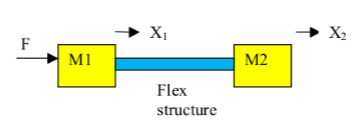
\includegraphics[width=0.5\linewidth]{./figures/flexStructure.png}
\end{center}
A dynamical system can be written as,
\begin{align}
  \left( M_{lump} + M_{rod} \right)
  \ddot U + 
  C_{rod} \dot U +
  K_{rod} U
  = 
  \begin{bmatrix}
    1 \\ 0
  \end{bmatrix}F,
\end{align}
where $U = \left[ x_1,x_2 \right]^T\in \mathbb{R}^2$ is the displacement of the two masses.
Given the density $\rho_r$ of the rod, the elastic modulus $E_r$ of the rod, the cross-sectional area $A_r$ of the rod, the length $L_r$ of the rod, and the masses $M_1$ and $M_2$, the system matrices can be written as,
\begin{align}
  M_{lump} &= 
  \begin{bmatrix}
    M_1 & 0 \\ 0 & M_1
  \end{bmatrix},~
  M_{rod} = 
  \dfrac{A_rL_r\rho_r}{6}
  \begin{bmatrix}
    2 & 1 \\ 1 & 2
  \end{bmatrix}\\
  C_{rod} &= \alpha K_{rod},~
  K_{rod} = 
  \dfrac{A_rE_r}{L_r}
  \begin{bmatrix}
    1 & -1 \\ -1 & 1
  \end{bmatrix}.
\end{align}
For simplicity, let
\begin{align}
  \dfrac{A_rL_r\rho_r}{6} = 1;~ \dfrac{A_rE_r}{L_r} = 1;~M_1=M_2=10;~\alpha = 0.1.
\end{align}
Finally, let the input be $F$ and the output be $x_2$.
\begin{parts}
  \part Obtain the state space model $\Sigma:= (A,B,C,D)$ of the system.
    Use Matlab to find the poles and zeros of the system.
  \part Use Matlab to find the transfer function of the system, and verify the locations of the poles and zeros
  \part The desired output acceleration of the system is $\ddot y = A\sin(\omega t)$. Choose $A$ such that the output reaches 1 after one period $T=10s$, and set it so that the acceleration reaches zero after $T$. Finally, obtain and plot the desired velocity and position as a function of time from $t_0=0$ to $t_f=T$.
  \part Choose your favourite feedback system to track the desired reference output (for example, LQR) and explain your design decisions.
  \part Simulate and plot the output tracking of the system with this feedback (for example, using LSIM in Matlab). What happens to the tracking performance if $T$ is varied?
  \part Find the internal dynamics of the system, then find the reference state trajectory $x_{ref}$ and the inverse input $u_{inv}$.
    Plot them, and describe how you found them.
  \part Simulate and plot the system with this feedforward input.
  \part Add the feedforward and feedback inputs together, and simulate the results in Matlab. Which setup has the best tracking performance (i.e., feedback, feedforward, feedback + feedforward)?
  \part Using the feedback + feedforward controller in the previous part, modify the system slightly before simulation (for example, modify $M_1$ and $M_2$ by $\pm 1\%$) in order to simulate uncertainty in the model parameters. Which setup has the best tracking performance (i.e., feedback, feedforward, feedback + feedforward)?
\end{parts}

\question[20] 
Estimate the resistance value starting from a series of repeated current and voltage measurements.
Assume the true relationship
\[
u_0(t) = R_0\, i_0(t), \qquad t=1,2,\ldots,N,
\]
where $u_0,i_0$ are the exact (noise–free) voltage and current.

Two different voltmeters are used, producing two data sets: one with low noise and one with high noise.

\begin{itemize}
  \item \textbf{Data generation.} Generate an experiment with $N$ measurements where
  $i_0$ is uniformly distributed in $[-0.01,\,0.01]~\mathrm{A}$ and $R_0=1250~\Omega$.
  The current is measured without errors, while the voltage measured by the two voltmeters is disturbed by independent, zero-mean, normally distributed noise $n_u$:
  \[
  n_u \sim \mathcal{N}(0,\sigma_u^2), \qquad
  \sigma_u^2 =
  \begin{cases}
  1,  & \text{(good voltmeter)},\\
  16, & \text{(bad voltmeter)}.
  \end{cases}
  \]
  Thus, with the measured signals
  \[
  i(t)=i_0(t), \qquad
  u(t)=u_0(t)+n_u(t), \qquad t=1,2,\ldots,2N,
  \]
  the first $N$ samples come from the good voltmeter and the next $N$ from the bad one.
\end{itemize}
\begin{parts}
  \part[5] \textbf{Weighted least-squares (WLS).} Derive the WLS estimate $\hat R$ of $R$ by minimizing
  \[
  V_{\mathrm{WLS}} = \frac{1}{2N}\sum_{t=1}^{2N} \frac{\big(u(t)-R\,i(t)\big)^2}{w(t)},
  \]
  where $w(t)$ is the variance of the voltage noise corresponding to sample $t$.
  Also, derive the \textbf{unweighted} least squares estimator, which minimizes,
  \begin{align}
    V_{\mathrm{LS}} =  \frac{1}{2N}\sum_{t=1}^{2N} {\big(u(t)-R\,i(t)\big)^2}
  \end{align}

  \begin{solution}
    To find the optimal $ \hat{R}_{WLE} $, we differentiate with respect to R and set the expression equal to 0, to find the given R.
    
    \begin{align*}
      \frac{ \partial V_{WLS} }{ \partial R } &= 2 \cdot \frac{ 1 }{ 2N } \sum_{ t=1 }^{ 2N } \frac{ i \left( u - Ri \right)  }{ w } \\
      &= \frac{ 1 }{ N } \sum_{ t=1 }^{ 2N } \frac{ i u  }{ w } - R\frac{ 1 }{ N } \sum_{ t=1 }^{ 2N } \frac{ i^2  }{ w } \\
      \frac{ 1 }{ N } \sum_{ t=1 }^{ 2N } \frac{ i u  }{ w } &= R\frac{ 1 }{ N } \sum_{ t=1 }^{ 2N } \frac{ i^2 }{ w} \\
      \hat{R}_{WLS} &= \frac{ \sum_{ t=1 }^{ 2N } \frac{ i(t)u(t) }{ w(t) } }{ \sum_{ t=1 }^{ 2N } \frac{ i(t)^2 }{ w(t) } }
    \end{align*}

    And for the LS method, without the weights added, we get

    \begin{align*}
      \frac{ \partial V_{LS} }{ \partial R } &= 2 \cdot \frac{ 1 }{ 2N } \sum_{ t=1 }^{ 2N } i \left( u - Ri \right) \\
      &= \frac{ 1 }{ N } \sum_{ t=1 }^{ 2N } iu - R \frac{ 1 }{ N } \sum_{ t=1 }^{ 2N } i^2  \\
      \frac{ 1 }{ N } \sum_{ t=1 }^{ 2N } iu &= R \frac{ 1 }{ N } \sum_{ t=1 }^{ 2N } i^2 \\
      \hat{R}_{LS} &= \frac{ \sum_{ t=1 }^{ 2N } iu }{ \sum_{ t=1 }^{ 2N } i^2 }
    \end{align*}
    
    And the question should be answered
    
  \end{solution}

  \part[5] Set $N=100$. Compute an estimate $\hat{R}$ $10^5$ times, using different data each time (according to the Data Generation procedure above), for both the LS and WLS procedures.
    Plot the resulting values of $\hat R$ in two histograms with an appropriate number of bins, one histogram for WLS and one for LS.
    Discuss the results.

    \begin{solution}
      There should be no surprise that the WLS estimates of the Ohms provide the most accurate ones. This happens because we have two voltimeters, and we give the voltimeter we trust the most, the most weight. This weight is given as the variance of the voltage noise ordered by the voltimeters. 

      \begin{center}
        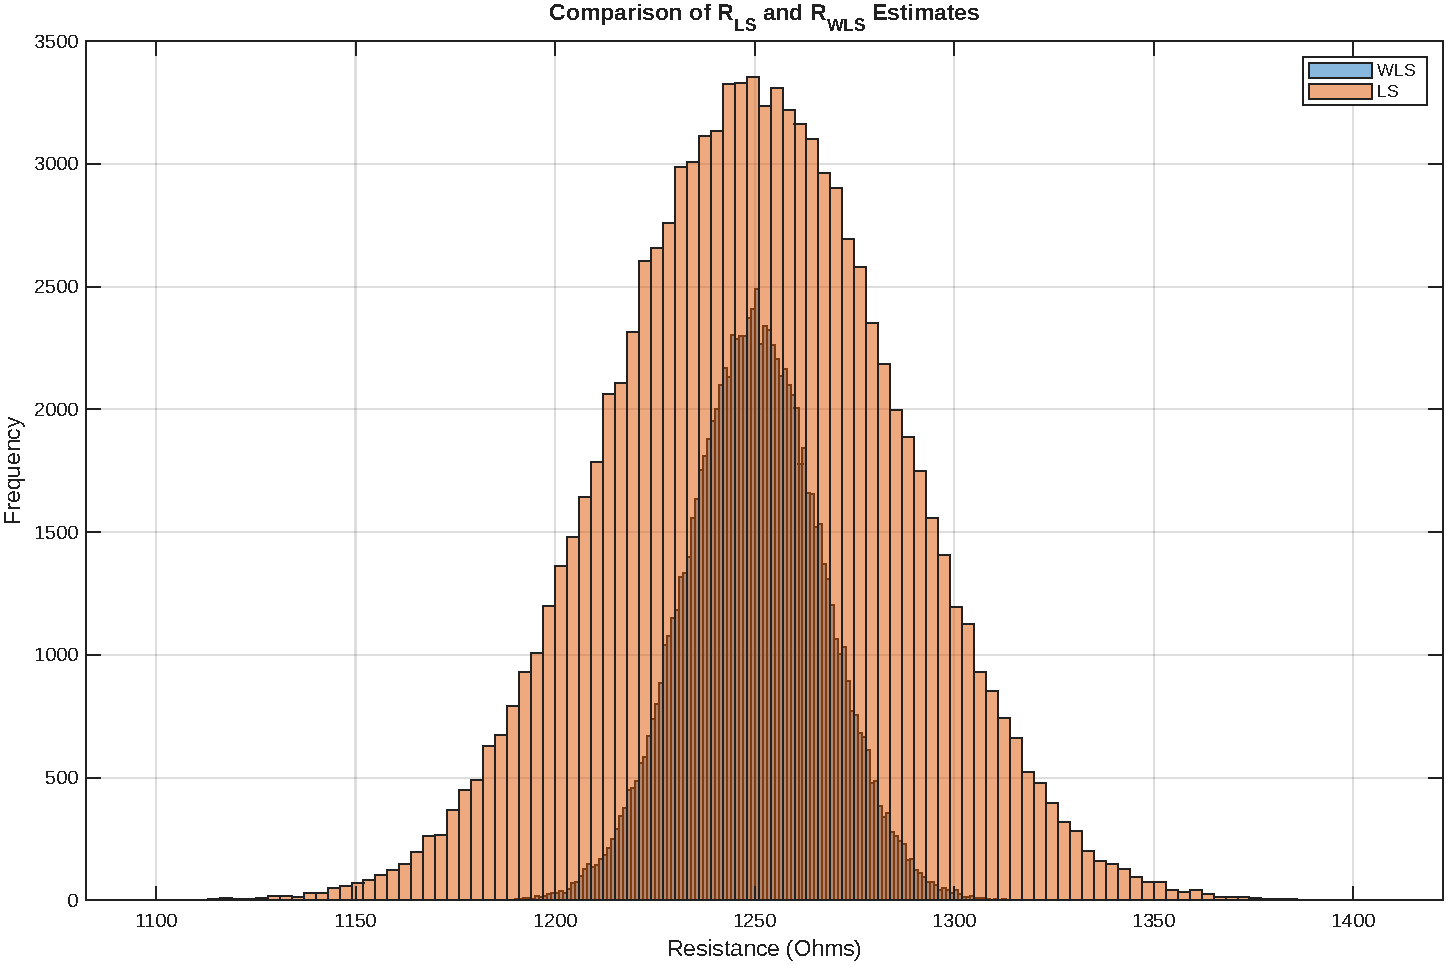
\includegraphics[width=1\linewidth]{Figure_6.pdf}
      \end{center}

      The estimation of $ \hat{R } $ over all the $ 10^5 $ experiments, leads to the figure above, which looks normally distributed, and indeed it obviously is, from the errors from the 2 voltimeters that are normally distributed

      \begin{center}
        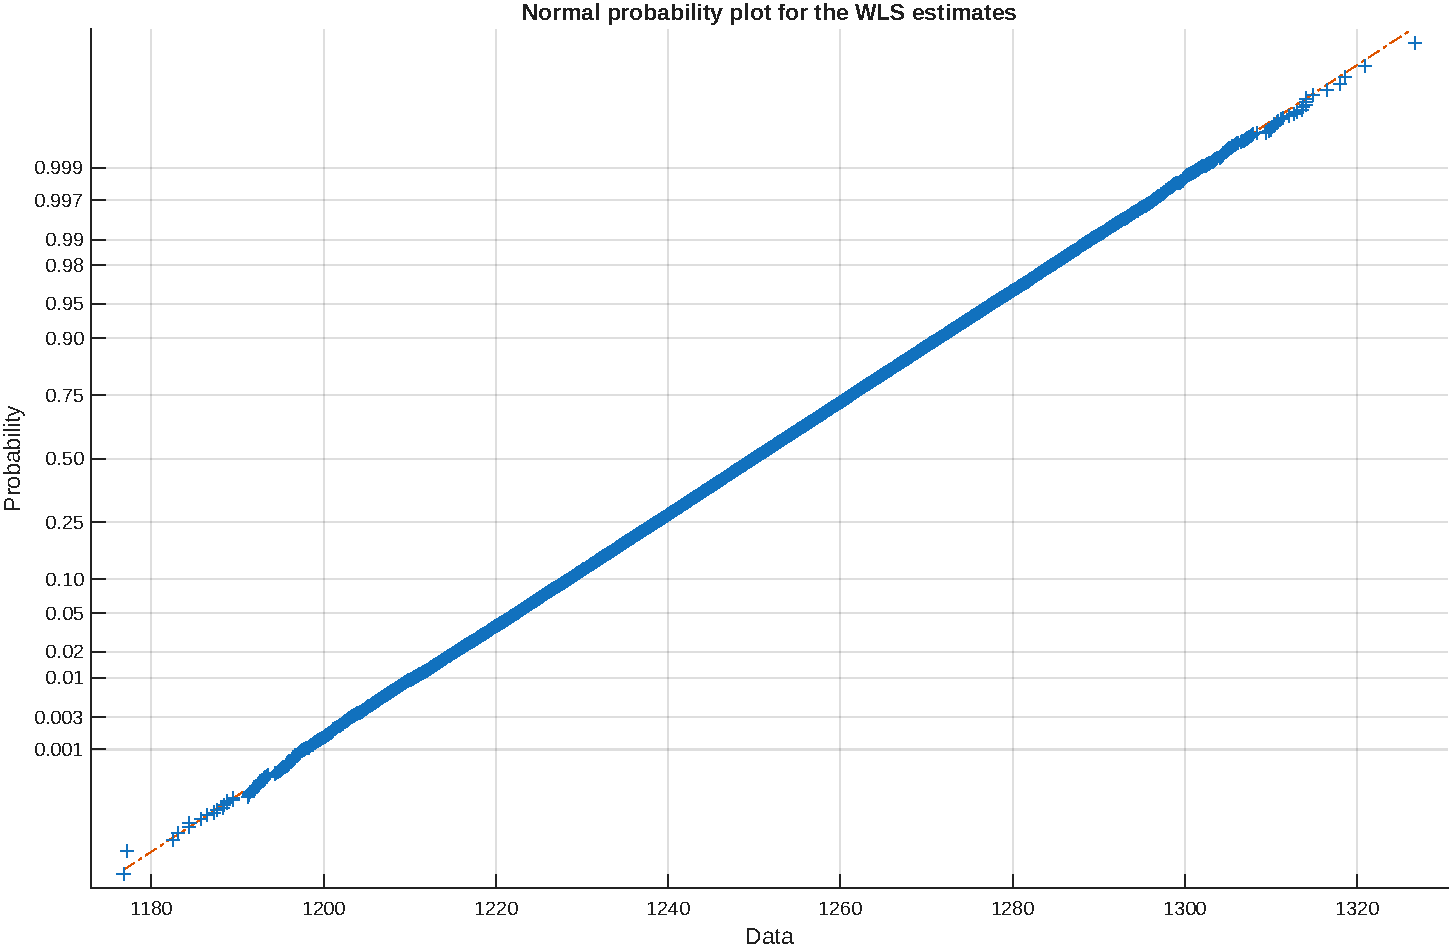
\includegraphics[width=0.8\linewidth]{normality_WLS.pdf}
      \end{center}
      \begin{center}
        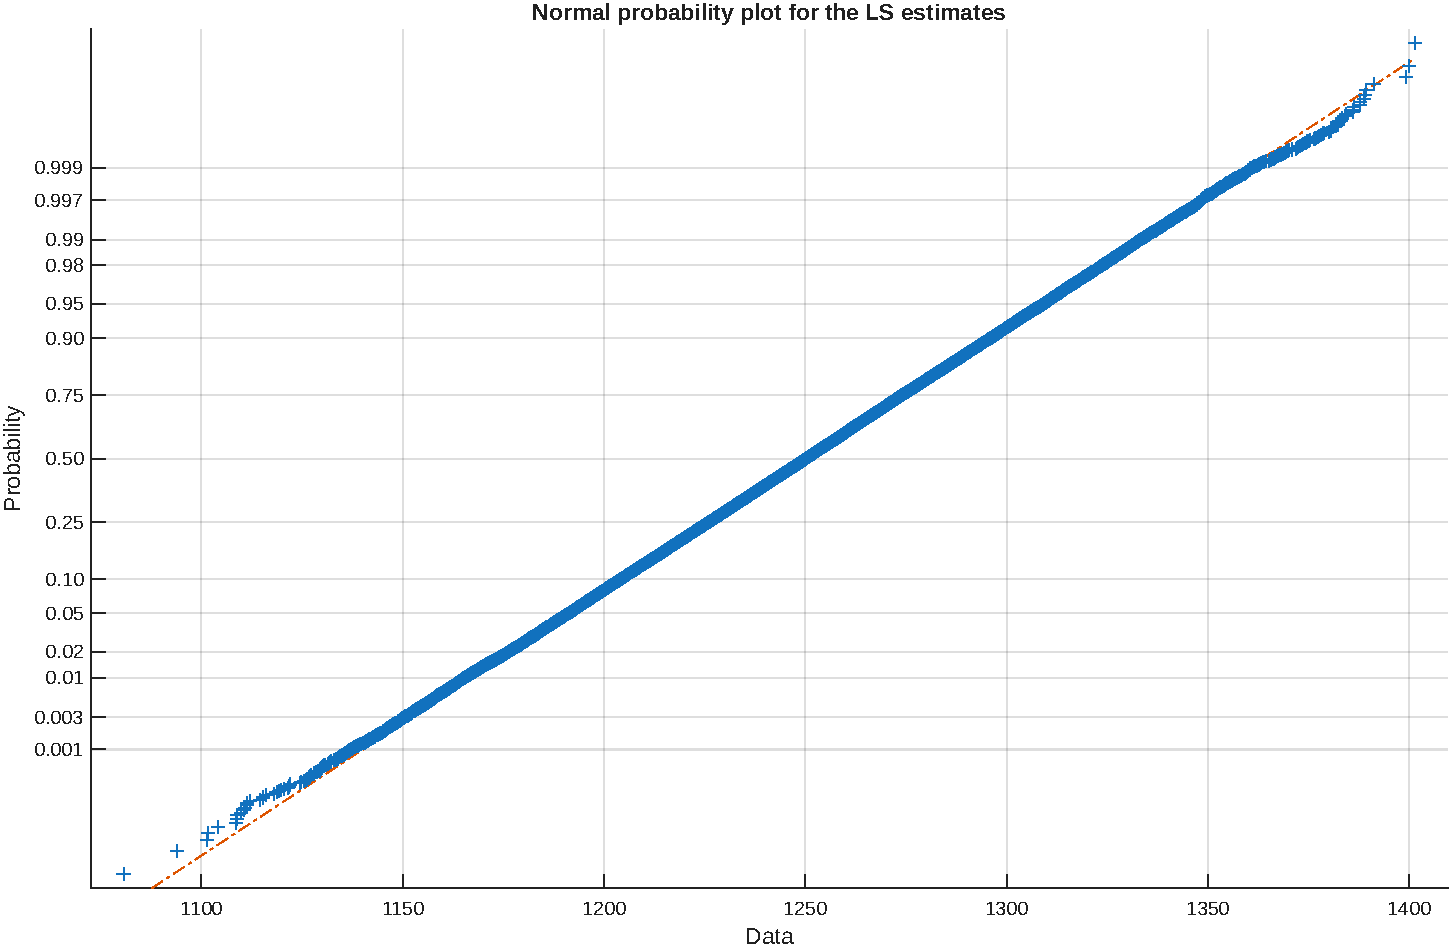
\includegraphics[width=0.8\linewidth]{normality_LS.pdf}
      \end{center}
      

      Basically, if the two arrays for the estimates, are closer to the straigt line with slope $ \frac{ 1 }{ 1320-1180 } = \frac{ 1 }{ 140 } $, the more normal it is distributed. The plots above confirms our belief.
    \end{solution}



  \part[10] Derive expressions for the variance of the WLS and the LS estimators. Compute the values of each based on the model parameters listed in the Data Generation procedure. Then, compute the sample variance of the estimates $\hat R$ in your experiments in part (a). Compare these to the expressions that you derived/computed. What would happen as the number of experiments increases from $10^5$?

  \begin{solution}
    To derive the variance of the estimators, we take the $ \hat{R}_{LS} $ and $ \hat{R}_{WLS} $ and set them as inputs to the function $ V(x) $
    
    \begin{align*}
      V(\hat{R}_{WLS}) &= V \left( \frac{ \sum_{ t=1 }^{ 2N } \frac{ i(t) u(t) }{ w(t) } }{ \sum_{ t=1 }^{ 2N } \frac{ i(t)^2 }{ w(t) } } \right) \\
      &=V \left( \frac{ \sum_{ t=1 }^{ 2N } \frac{ i(t) \left( R_0i_0(t) + n_u(t) \right)  }{ w(t) } }{ \sum_{ t=1 }^{ 2N } \frac{ i(t)^2 }{ w(t) } } \right) \\
      &= V \left( \frac{ \sum_{ t=1 }^{ 2N } \frac{ i(t)R_0i_0(t) }{ w(t) } }{ \sum_{ t=1 }^{ 2N } \frac{ i(t)^2  }{ w(t) } } + \frac{ \sum_{ t=1 }^{ 2N } \frac{ i(t) n_u(t) }{ w(t) } }{ \sum_{ t=1 }^{ 2N } \frac{ i(t)^2 }{ w(t) } } \right) 
    \end{align*}

    
    Since $ i(t) = i_0(t) $ is the \textbf{\textit{true}} current, we can substitute that into the first fraction and get 

    \begin{align*}
      V(\hat{R}_{WLS} &= V(R_0) + \frac{ \sum_{ t=1 }^{ 2N } \frac{ i(t)^2 V(n_u(t) }{ w(t)^2 } }{ \left( \sum_{ t=1 }^{ 2N } \frac{ i(t)^2 }{ w(t) } \right)^2  }
    \end{align*}
    And since $ V(n_u(t)) = w(t) $, we get
    
    \begin{align*}
      V(\hat{R}_{WLS}) &= \frac{ \sum_{ t=1 }^{ 2N } \frac{ i(t)^2 }{ w(t) } }{ \sum_{ t=1 }^{ 2N } \frac{ i(t)^4 }{ w(t)^2 } }\\
      &= \frac{ 1 }{ \sum_{ t=1 }^{ 2N } \frac{ i(t)^2 }{ w(t) } }
    \end{align*}
    
    Which is the final expression. Its important to note that for a linear equation $ a+bx $, then $ V(a+bx) = b^2V(x) $ where x is a random variable, which is why the $ R_0 $ term disappears
    
    Now for the derivation of $ \hat{R}_{LS} $ 

    \begin{align*}
      V(\hat{R}_{LS}) &=  V \left( \frac{ \sum_{ t=1 }^{ 2N } i(t)u(t) }{ \sum_{ t=1 }^{ 2N } i(t)^2 } \right) \\
      &= V \left( \sum_{ t=1 }^{ 2N } \frac{ i(t) \left( R_0i_0(t) + n_u(t) \right)  }{ i(t)^2 } \right)  \\
      &= V \left( \sum_{ t=1 }^{ 2N } \frac{ i(t) R_0 + i(t)^2 n_u(t) }{ i(t)^2 } \right) \\
      &= V(R_0) + \sum_{ t=1 }^{ 2N } \frac{ i(t)^2V(n_u(t) }{ i(t)^4 } \\
      &= \frac{ 1 }{ \sum_{ t=1 }^{ 2N } \frac{ i(t)^2 }{ w(t) } }
    \end{align*}
    from the same reasoning that $ V(n_u(t)= w(t) $ 
    
  \end{solution}
\end{parts}

\question[20] \textbf{Least-Squares Identification of a One-Parameter Linear System.}
Consider the discrete-time system
\[
y_k = a\,y_{k-1} + b\,u_{k-1} + e_k, \qquad k = 2, \ldots, N,
\]
where
\begin{itemize}
  \item \(y_k\) is the measured output,
  \item \(u_k\) is the known input,
  \item \(e_k\) is a zero-mean white noise sequence,
  \item \(a,b\) are unknown parameters to be estimated.
\end{itemize}
Stack all samples \(k=2,\ldots,N\) to obtain
\[
\mathbf{y} = \Phi\,\theta + \mathbf{e},
\]
with
\begin{align}
\Phi =
\begin{bmatrix}
y_1 & u_1\\
y_2 & u_2\\
\vdots & \vdots\\
y_{N-1} & u_{N-1}
\end{bmatrix},
\qquad
\theta =
\begin{bmatrix}
a\\
b
\end{bmatrix},
\qquad
\mathbf{y} =
\begin{bmatrix}
y_2\\
y_3\\
\vdots\\
y_N
\end{bmatrix},
\qquad
\mathbf{e} =
\begin{bmatrix}
e_2\\
e_3\\
\vdots\\
e_N
\end{bmatrix}.
\label{eq:model}
\end{align}

\begin{parts}
\part[5]
By minimizing the sum of squared residuals
\[
V(a,b) = \sum_{k=2}^N \big(y_k - a\,y_{k-1} - b\,u_{k-1}\big)^2,
\]
show that the optimal parameters satisfy the \emph{normal equations}
\[
\Phi^\top \Phi\,\hat{\theta} = \Phi^\top \mathbf{y},
\]
leading to the closed-form least-squares solution
\begin{align}
  \boxed{\hat{\theta} = (\Phi^\top \Phi)^{-1}\Phi^\top \mathbf{y}.}\label{eq:ls}
\end{align}

\begin{solution}
  To derive the optimal parameters that satisfy the normal equations, we see first that from the exercise, we are given that we have dropped the error terms in the sum. And when we stack all the $ y_k, u_k, $ and all a, b that shall be  estimated, we get the sum thats given in the exercise. In quadratic form, this turns to

  \begin{align*}
    r &= y - \Phi \theta\\ 
    V(\theta) &= r^Tr\\ 
    &= \left( y - \Phi \theta \right) ^T \left( y - \Phi \theta \right) \\
    &= y^Ty - y^T \Phi \theta - \left( \Phi \theta \right)^T y + \left( \Phi \theta \right)^T \left( \Phi \theta \right) \\
    &= y^Ty - 2 \theta^T \Phi ^T y + \theta^T \Phi^T \Phi \theta
  \end{align*}
  


  
  And now we have to find the optimal parameters a, b that find the minimized sum of squared residuals

  \begin{align*}
    \frac{ \partial V(\theta) }{ \partial \theta } &= 0 - 2 \Phi ^T y + 2 \Phi^T \Phi \theta =0\\
    2\left( \Phi ^T \Phi \right)\hat{\theta} &=  2\Phi^T y \\
    \hat{\theta} &= \left( \Phi ^T \Phi \right) ^{-1} \Phi^T y
  \end{align*}
  This assumes of course that $ \Phi^T \Phi $ is invertible. I will get to this more in 3 c). But all in all, I think the exercise is solved.
  

\end{solution}

\part[10] Set $N=100$, $a=0.2$ and $b=-0.25$, and $e_k\sim \mathcal{N}(0,0.5)$, and consider the following input sequences:
\begin{itemize}
  \item a random input that is 1 half the time, and -1 half the time: 
    \begin{align}
      u_k \sim 
    \begin{cases}
      1 & {p=0.5}\\
      -1 & {p=-0.5}
    \end{cases}
    \end{align}
  \item a random uniform input:
    \begin{align}
      u_k \sim \textbf{randu[-1,1]}
    \end{align}
  \item a gaussian input with mean zero and variance 1:
    \begin{align}
      u_k \sim \mathcal{N}(0,1)
    \end{align}
\end{itemize}

For each input type, perform the following:
\begin{itemize}
  \item Generate $\mathbf{y}$ using Equation~\eqref{eq:model}
  \item Generate $\hat\theta$ using Equation~\eqref{eq:ls}
  \item Repeat this process $10^5$ times
\end{itemize}
Plot histograms for $\hat{a}$ and for $\hat{b}$ for the different input types on the same plot. Which input type yields the lowest variance estimate?

\begin{solution}
  Here is the histogram plots for the different a and b:

  \begin{center}
    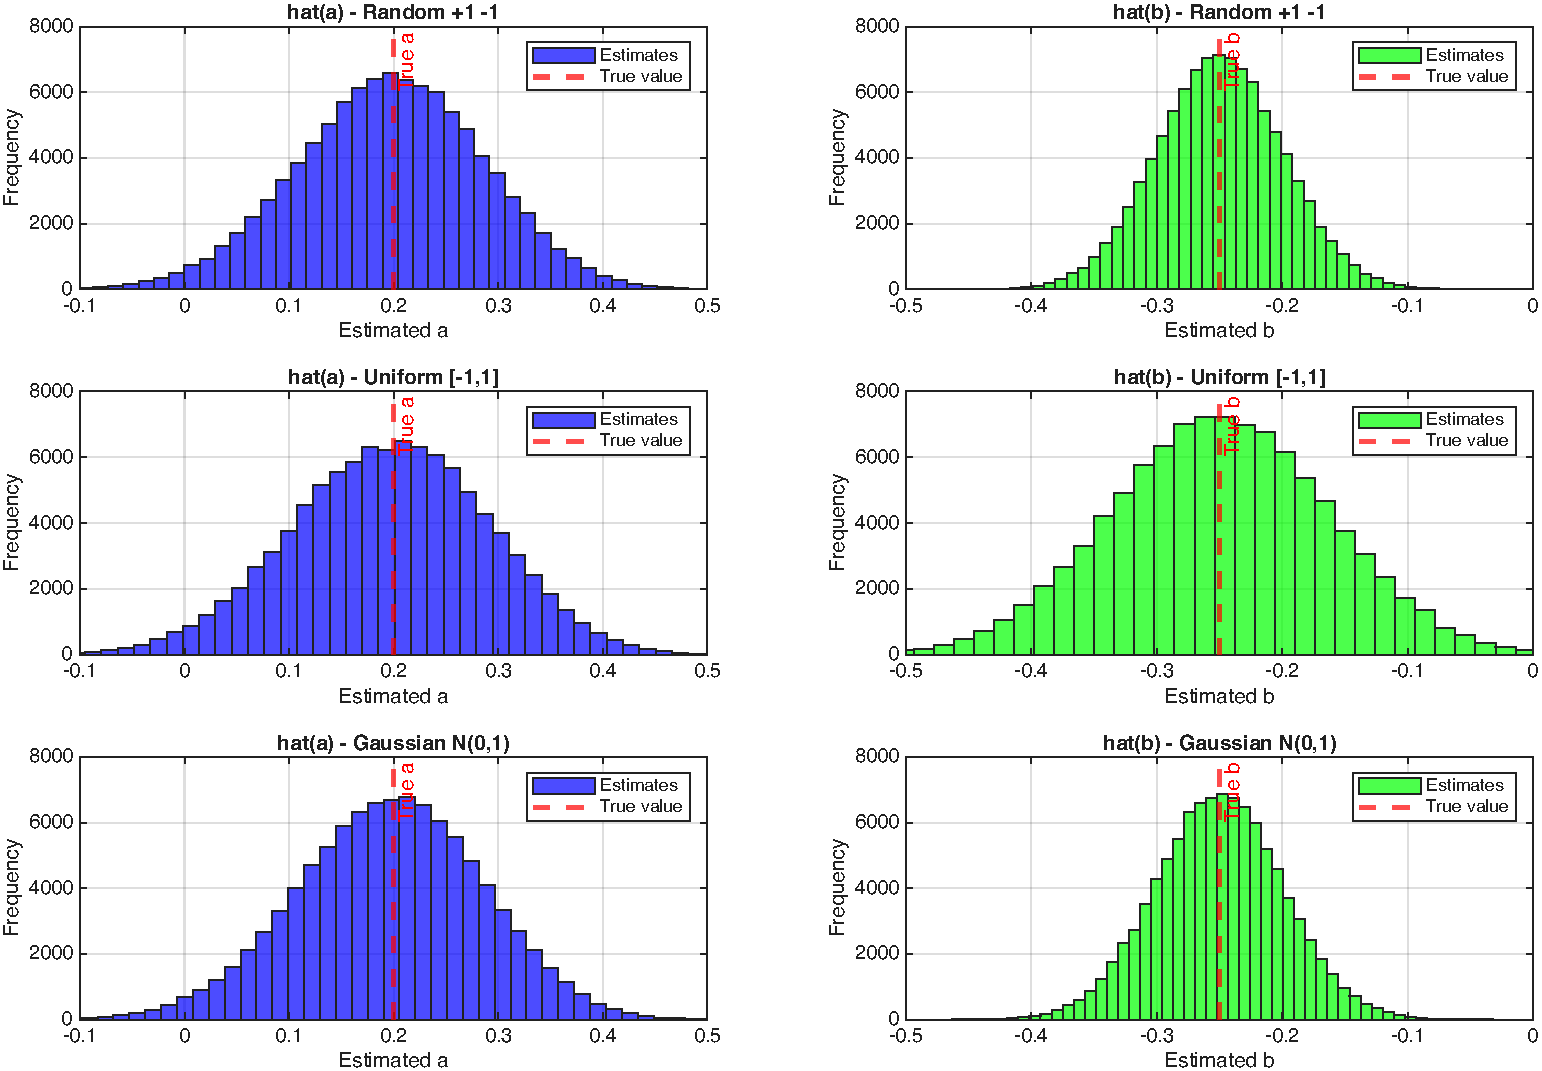
\includegraphics[width = 1\linewidth]{./figures/figure_exc_3b_A3.pdf}
  \end{center}

  I will refer to the different control series generation processes like the following:

  \begin{itemize}
  \item \textbf{\textit{Method 1}}: a random input that is 1 half the time, and -1 half the time: 
    \begin{align}
      u_k \sim 
    \begin{cases}
      1 & {p=0.5}\\
      -1 & {p=-0.5}
    \end{cases}
    \end{align}
  \item \textbf{\textit{Method 2}}: a random uniform input:
    \begin{align}
      u_k \sim \textbf{randu[-1,1]}
    \end{align}
  \item \textbf{\textit{Method 3}}: a gaussian input with mean zero and variance 1:
    \begin{align}
      u_k \sim \mathcal{N}(0,1)
    \end{align}
\end{itemize}

  I also gather that the empirical variance of the $ \hat{a} $ and $ \hat{b} $ arrays vary between the method 1 and method 3. The following table displays the variance of said arrays, where column i is either the $ \hat{a} $ array or the $ \hat{b} $ array, and the column i is $ method_i $ 

  \begin{table}[h]
\centering
\begin{tabular}{lcc}
\hline
Input Type & Var(\^{a}) & Var(\^{b}) \\
\hline
Method 1 & 0.007833 & 0.002547 \\
Method 2 & 0.009062 & 0.007751 \\
Method 3 & 0.007848 & 0.002587 \\
\hline
\end{tabular}
\end{table}

From this, we see that method 2 is without a doubt the worst. It is relatively close between method 1 and method 2 having the lowest variance implication on the coefficient estimates $ \hat{a} $ and $ \hat{b} $.

It comes to the point where it differs between each time I run the code. 

\end{solution}

\part[5] Discussion
\begin{enumerate}
  \item Under what conditions is \(\Phi^\top\Phi\) invertible?
  \begin{solution}
      $ \Phi^T \Phi $ is invertible if and only if the following is satisfied; The columns of $ \Phi^T \Phi $ have full rank. The only case where this would not happen, was if the controls $ u_k = 0 \forall k$. This is unlikely in practice 
    \end{solution} 
  \item What happens if the input \(u_k\) is constant?
  \begin{solution}
      If one of the controls are constant, I dont see any much affection on the series y. But if $ u_k=0 \forall k $ then the matrix $ \Phi^T \Phi $ is non-invertible. I mentioned this earlier. In this case, the estimates $ \hat{a} $ and $ \hat{b} $ are all zero. This is because the equation

      \[
          \hat{\theta} = \left( \Phi^T \Phi \right) ^{-1} \Phi^T y
      \]

      would not exist, due non-invertible property of the $ \Phi^T \Phi $ matrix
      
  \end{solution}
  \item How would correlated noise \(e_k\) affect the bias of the estimates?
  \begin{solution}
    FDGDS
  \end{solution}
\end{enumerate}


\end{parts}
\end{questions}
\end{document}